El punto $E$ indica la situación inicial de ambos consumidores. En este punto, el agente $A$ tiene una dotación de $(1,2)$; mientras que el $B$ una de $(2,1)$. La curva de contrato viene dada por la línea gruesa y el área morada señalada en el siguiente gráfico.

\begin{center}
	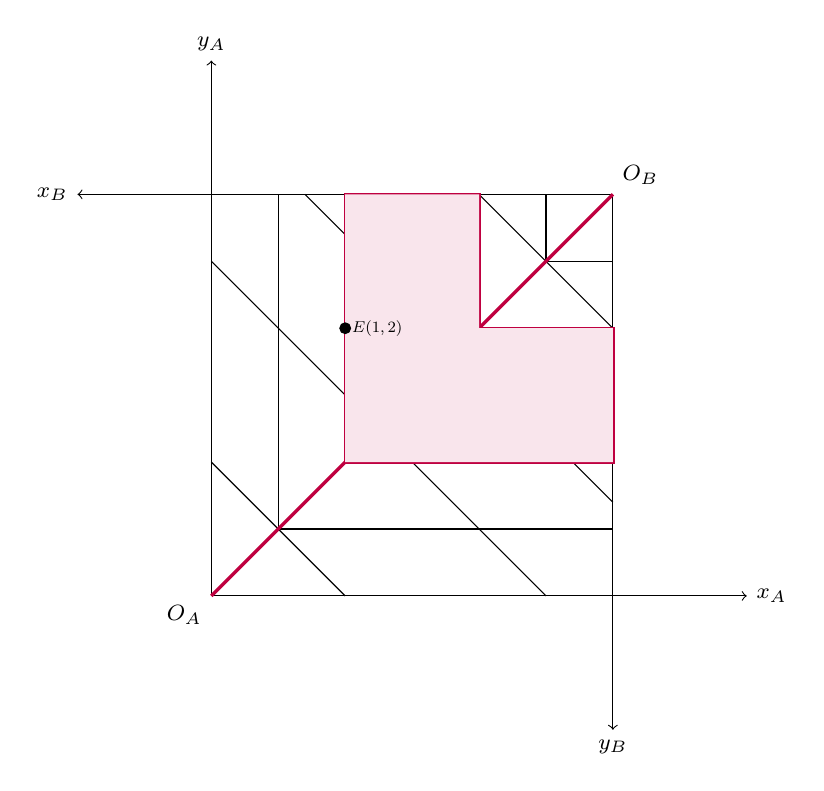
\begin{tikzpicture}[scale=1.7]
		% Formato de CAJA
		\draw[->] (0,0) node[align=center, below left] {\footnotesize $O_A$} -- (0,4) node[align=center, above] {\footnotesize $y_A$};
		\draw[->] (0,0) -- (4,0) node[align=center, right] {\footnotesize $x_{A}$};
		
		\draw[->] (3,3) node[align=center, above right] {\footnotesize $O_B$} -- (-1,3) node[align=center, left] {\footnotesize $x_{B}$};
		\draw[->] (3,3) -- (3,-1) node[align=center, below] {\footnotesize $y_{B}$};
		
		% 
		
		% Curvas de indiferencia
		\draw (0.5,3) -- (0.5,0.5) -- (3,0.5);
		\draw (2.5,3) -- (2.5,2.5) -- (3,2.5);
		
		\draw (2,3) -- (3,2);
		\draw (0,2.5) -- (2.5,0);
		\draw (0.7,3) -- (3,0.7);
		\draw (0,1) -- (1,0);
		
		% Curva de contrato       
		\draw [purple, very thick] (0,0)  -- (1,1);
		\draw [purple, very thick] (2,2)  -- (3,3);
		\draw [purple, very thick] (1,1)  -- (1,3) -- (2,3) -- (2,2) -- (3,2) -- (3,1) -- (1,1);
		\fill [color=purple!10](1,1)  -- (1,3) -- (2,3) -- (2,2) -- (3,2) -- (3,1) -- (1,1);
		
		% Punto
		\draw[black, fill=black] (1,2) circle[radius=0.04] node[align=center, right, scale = 0.25mm] {\footnotesize $E(1,2)$};
	\end{tikzpicture}
\end{center}